\let\negmedspace\undefined
\let\negthickspace\undefined

\documentclass[journal]{IEEEtran}
\usepackage[a5paper, margin=10mm, onecolumn]{geometry}
%\usepackage{lmodern} % Ensure lmodern is loaded for pdflatex
\usepackage{tfrupee} % Include tfrupee package

\setlength{\headheight}{1cm} % Set the height of the header box
\setlength{\headsep}{0mm}     % Set the distance between the header box and the top of the text

\usepackage{gvv-book}
\usepackage{gvv}
\usepackage{cite}
\usepackage{amsmath,amssymb,amsfonts,amsthm}
\usepackage{algorithmic}
\usepackage{graphicx}
\usepackage{textcomp}
\usepackage{xcolor}
\usepackage{txfonts}
\usepackage{listings}
\usepackage{enumitem}
\usepackage{mathtools}
\usepackage{gensymb}
\usepackage{comment}
\usepackage[breaklinks=true]{hyperref}
\usepackage{tkz-euclide} 
\usepackage{listings}
% \usepackage{gvv}                                        
\def\inputGnumericTable{}                                 
\usepackage[latin1]{inputenc}                                
\usepackage{color}                                            
\usepackage{array}                                            
\usepackage{longtable}                                       
\usepackage{calc}                                             
\usepackage{multirow}                                         
\usepackage{hhline}                                           
\usepackage{ifthen}                                           
\usepackage{lscape}
\begin{document}

\bibliographystyle{IEEEtran}
\vspace{3cm}

\title{4.10.10}
\author{EE25BTECH11010 - Arsh Dhoke}
{\let\newpage\relax\maketitle}

\renewcommand{\thefigure}{\theenumi}
\renewcommand{\thetable}{\theenumi}
\setlength{\intextsep}{10pt}
\numberwithin{equation}{enumi}
\numberwithin{figure}{enumi}
\renewcommand{\thetable}{\theenumi}

\parindent 0px
\textbf{Question}:\\
Find the distance of the point (-1,-5,-10) from the point of intersection of the line $\vec{r}=2\vec{i}-\vec{j}-2\vec{k}+ \lambda(3\vec{i}+4\vec{j}+2\vec{k})$ and the plane $\vec{r}\cdot(\vec{i}-\vec{j}+\vec{k})=5$.

\solution \\

On comparing equation of line with $\vec{x}=\vec{a}+ \lambda\vec{b}$
and equation of plane with $\vec{n}^T\vec{x}=c$ we get: \\

\begin{tabular}{|c|c|}
\hline
\textbf{Name} & \textbf{Value} \\ \hline
$\vec{A}$ & $\myvec{2 & 1 \\0 & 3}$ \\ \hline
\end{tabular}





\begin{align}
    \vec{n}^T\vec{x}=c
\end{align}

\begin{align}
    \vec{n}^T(\vec{a}+ \lambda\vec{b})=c
\end{align}

\begin{align}
    \lambda=\frac{c-\vec{n}^T\vec{a}}{\vec{n}^T\vec{b}}
\end{align}

\begin{align}
\vec{x}=\vec{a}+ \brak{\frac{c-\vec{n}^T\vec{a}}{\vec{n}^T\vec{b}}}\vec{b}    
\end{align}

\begin{align}
    \vec{n}^T\vec{a}=\myvec{1 & -1 & 1}\cdot\myvec{2 \\ -1 \\ -2}
    &=1
\end{align}

\begin{align}
    \vec{n}^T\vec{b}=\myvec{1 & -1 & 1}\cdot\myvec{3 \\ 4 \\ 2}
    &=1
\end{align}

Substituting given values in (0.4) we get:
\begin{align}
    \vec{x}=\myvec{14 \\ 15 \\ 6}
\end{align}

Distance between $\vec{P}$ and $\vec{x}$ :



    
$\norm{\vec{P}-\vec{x}}=\sqrt{15^2 + 20^2 + 16^2}
= \sqrt{225 + 400 + 256}
= \sqrt{881}$


\begin{figure}[ht!]
\centering
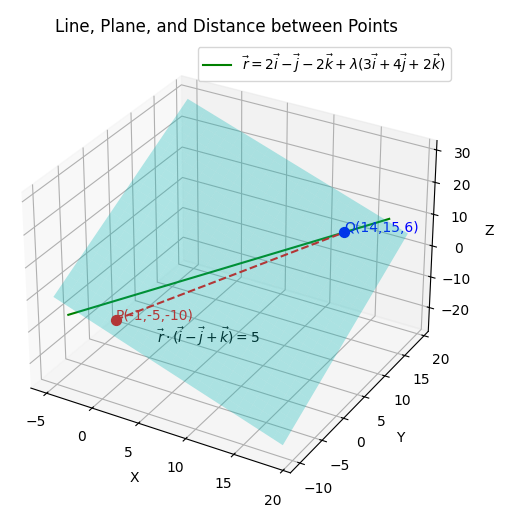
\includegraphics[height=0.6\textheight, keepaspectratio]{figs/q8.png}
\captionof{figure}{Graph}
\end{figure}
\end{document}